\chapter{Implementierung}
Im folgenden Kapitel wird die praktische Implementierung der in der Arbeit erarbeiteten Methode beschrieben. Die Implementierung umfasst dabei die Schnittstelle zum Nutzer, sowie die Erhebung, Verarbeitung und Persistenz von relevanten Daten.
\section{Backend}
Für die Implementierung der Arbeit wurde ein Backend konzipiert, welches Informationen und Bilder von Verkehrskameras für Clients vorenthält. 
Das Ziel ist es dabei, Daten der Straßenverkehrszentrale regelmäßig anzufragen und für den Client zu persistieren. 
Somit wird ermöglicht, dass der Client auch auf ältere Datensätze der Straßenverkehrszentrale zugreifen kann. 
Weiterhin ermöglicht das Backend die Daten in einem möglichst kompakten Format an den Client zu senden, damit auch über schwache Netzwerkverbindungen die Daten empfangen können. 
\subsection{Infrastruktur}
\label{sec:infrastructure}
Im Rahmen der Implementierung des Backends wurden diverse Anforderungen an die zu verwendenden Technologien beachtet. 
So soll die resultierende Anwendung auf dem Apache Server eines geteilten Webhosts laufen. 
Der Apache Server des Webhosts erlaubt das Ausführen von PHP-Skripten, welche für das Ansteuern von Anfragen und die Verarbeitung von Daten der Straßenverkehrszentrale Baden-Württemberg verwendet werden können. 

Für die Persistenz von Daten besitzt der Webhost alternativ zum Dateisystem auch eine MySQL-Datenbank.
Die Datenbank ist für die Implementierung besser geeignet als das Dateisystem, da sie Transaktionen sowie eine relationale Abbildung der  Datensätze ermöglicht.
So ermöglicht die Datenbank auch das einfache Abspeichern von Metadaten für Verkehrskameras und die Vernetzung zwischen Metadaten und Kamerabildern über Fremdschlüssel.

Ein weiterer Grund warum für den Anwendungsfall die Datenbank dem Dateisystem zu bevorzugen ist, ist, dass Datensätze einfach und schnell geordnet und gefiltert werden können.
Dies wird über die SQL-Sprache ermöglicht, die sowohl "`SELECT FROM WHERE"'-Klauseln sowie Aggregationsfunktionen wie "`SUM"' oder "`MAX"' für das Filtern von Datensätzen bietet.

Auf Abbildung~\ref{fig:serverarch} ist zu sehen, dass die Verbindung zum Client über das HTTP-Protokoll verläuft. 
Der Vorteil ist hierbei, dass das Protokoll bereits von dem Apache Server unterstützt wird und eine Verschlüsselung über TLS eingesetzt werden kann.

Ein weiterer Bestandteil der Backend-Infrastruktur ist der Cron-Daemon des Linux Betriebssystem des Host-Systems.
Über diesen lassen sich periodisch wiederholende Aufgaben einplanen, welche für das Backend nützlich sein könnten.
Ein Beispiel hierfür ist das regelmäßige Abfragen von Bildern einer Verkehrskamera der Straßenverkehrszentrale.

Die letzte Komponente der Infrastruktur ist die Applikation "`cURL"', die sich auf dem Betriebssystem des Hosts befindet.
cURL unterstützt die Übertragung von Daten über diverse Protokolle und lässt sich auch über Schnittstellen anderen Programmen und Programmiersprachen kontrollieren.
So ermöglicht dies auch das Anstoßen von HTTP-Anfragen über PHP-Skripte des Apache Servers.
cURL bietet zusätzlich auch die Funktionalität verschiedene Parameter der Anfragen einzustellen.
Einstellbare Parameter umfassen dabei unter anderem:
\begin{itemize}
\item{HTTP-Header (auch Referer-Header)}
\item{Timeout der Anfrage}
\item{Überprüfung von SSL-Zertifikaten (z.B. bei HTTPS)}
\item{Empfangen von spezifischen Headern (z.B. Last-Modified)}
\end{itemize}
\begin{figure}[hp]
   \centering
     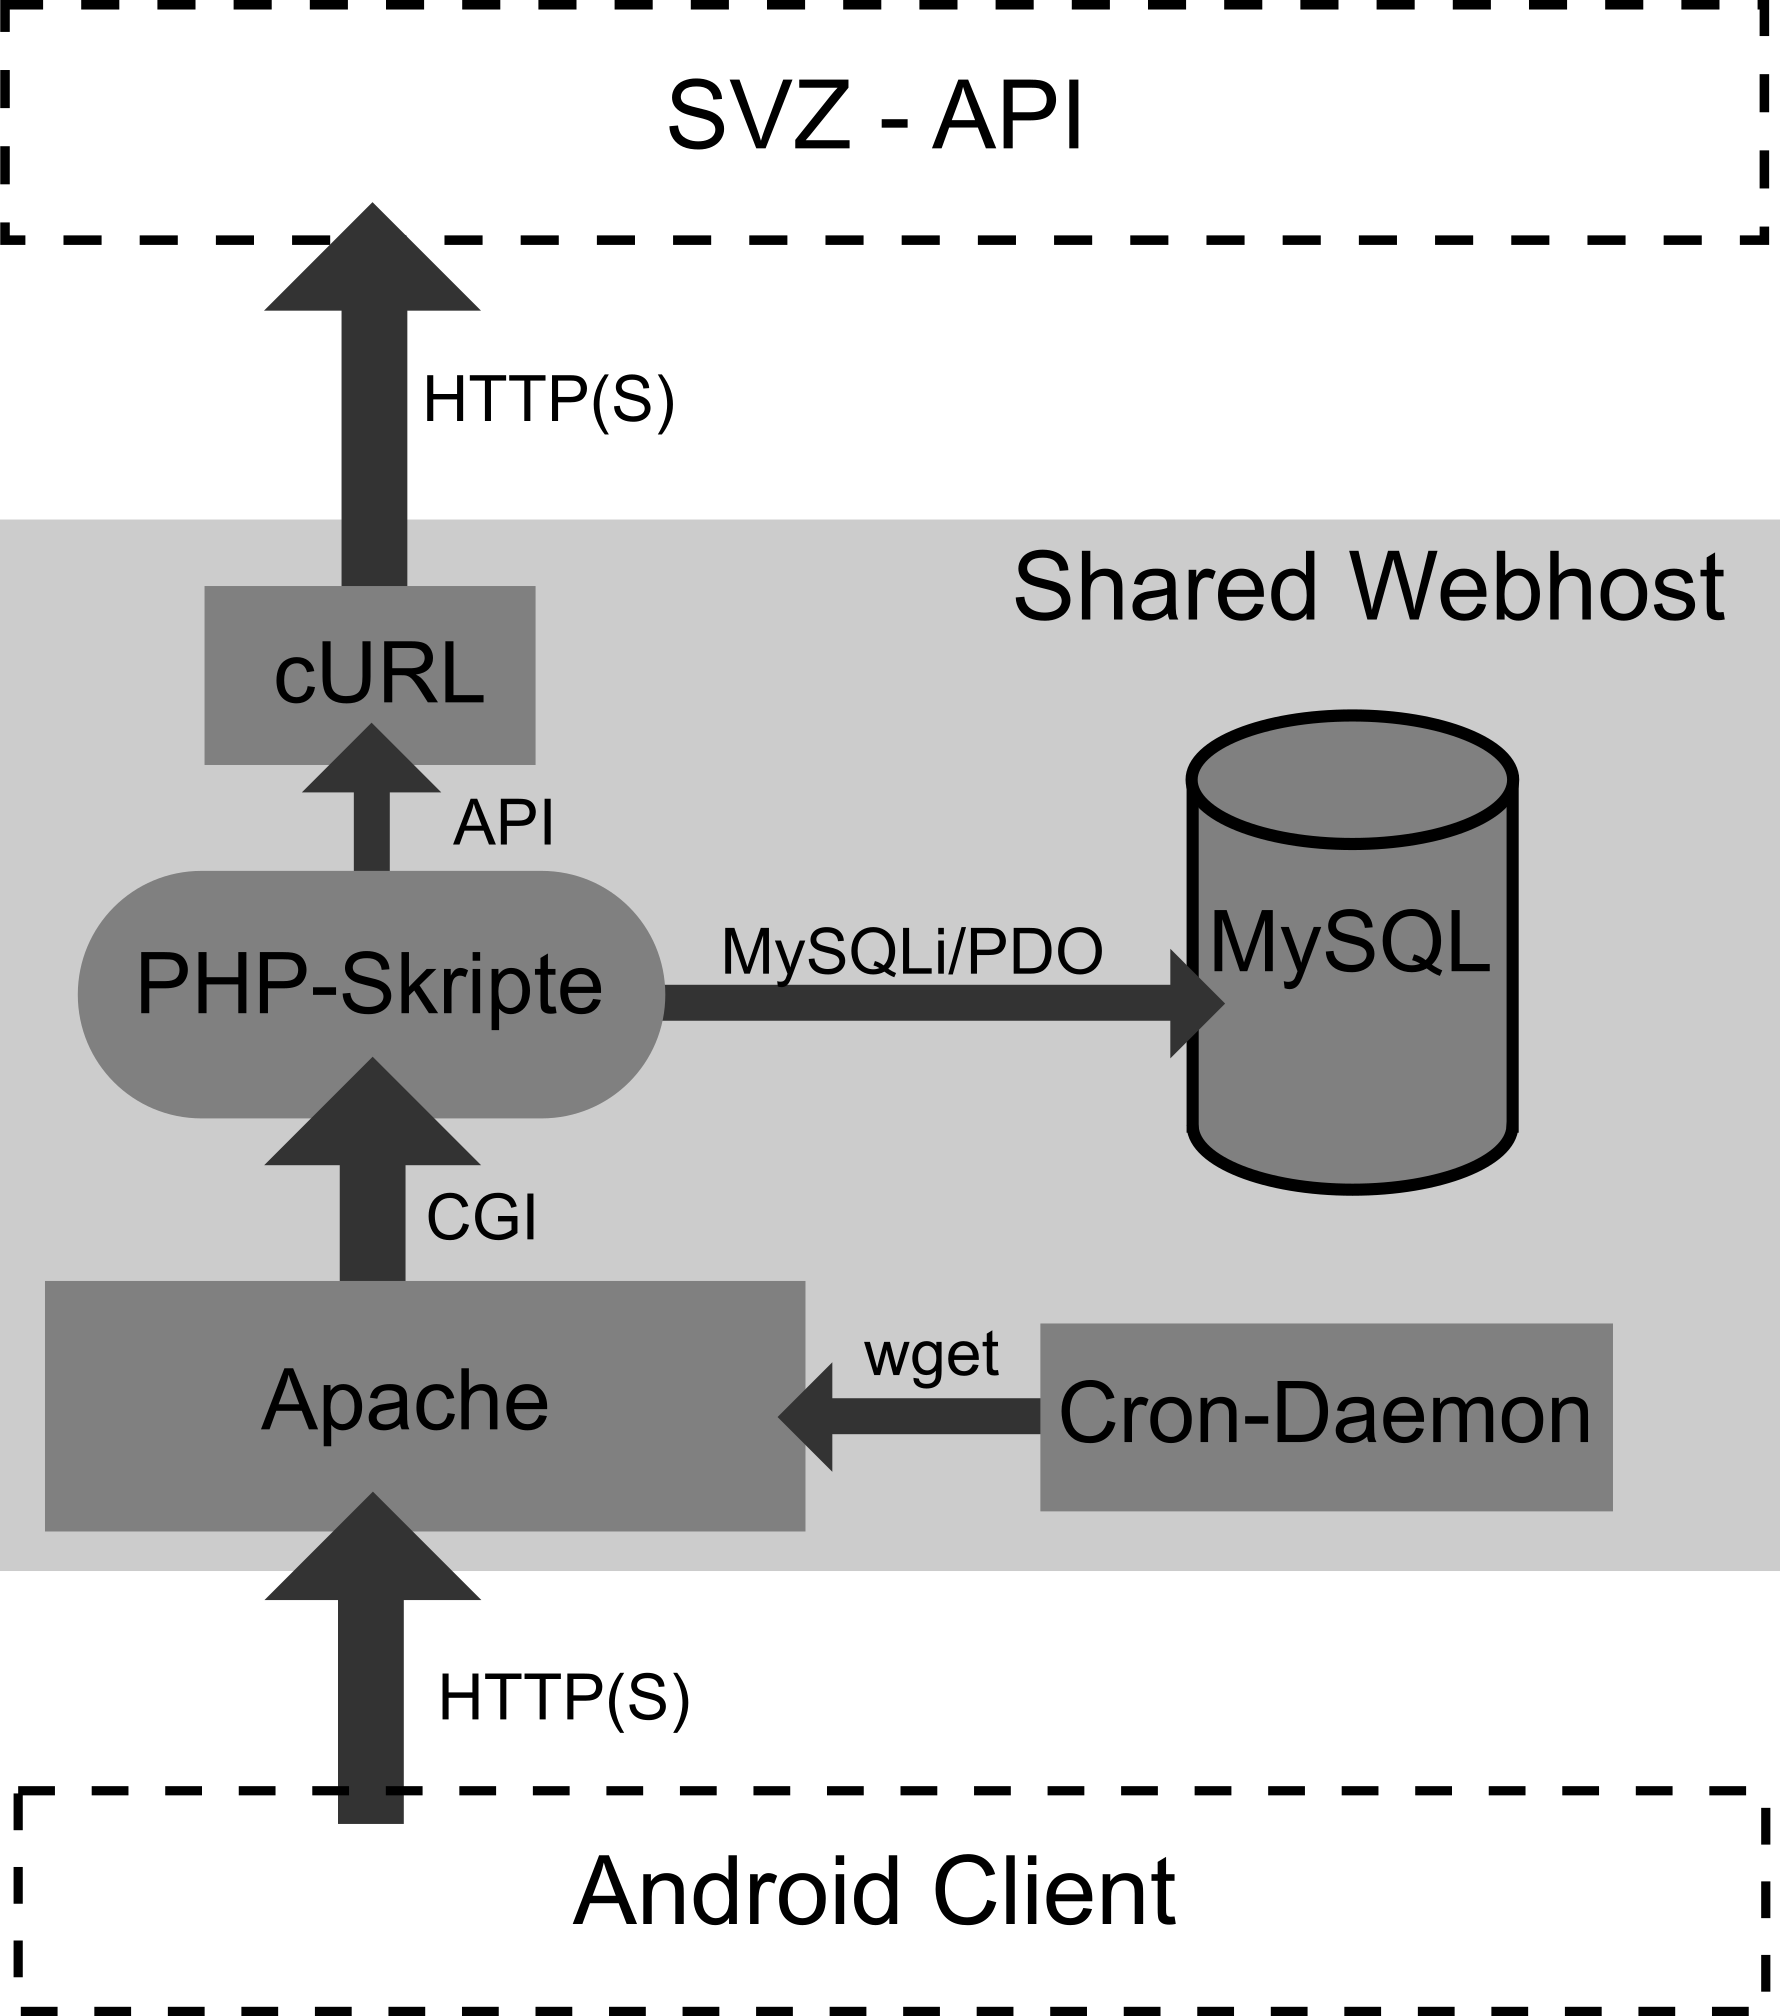
\includegraphics[width=13cm]{Bilder/server-arch} \\
 \caption{Server Architektur}
 \label{fig:serverarch}
\end{figure}
\newpage
\subsection{Datenerhebung}
\label{sec:datenerhebung}
Die Erhebung von benötigten Daten erfolgt durch HTTP-Anfragen an den Server der Straßenverkehrszentrale. Diese können mithilfe der cURL-API in PHP angestoßen werden.

Informationen über die jeweiligen Kameras werden über den SVZ-Server in verschieden Formaten bereitgestellt. So sind die Metadaten der Kameras als Textdatei abgespeichert, während die Bilder direkt im JPEG-Format abgerufen werden können. Unter Metadaten der Verkehrskameras sind folgende Informationen zu verstehen: 
\begin{itemize}
\item{Eine eindeutige alphanumerische Kamerakennung}
\item{Die entsprechende Autobahnkennung}
\item{Name der nächsten Ausfahrt mit Autobahnkennung}
\item{Position der Kamera}
\end{itemize}
Die Metadaten der Kameras müssen nur einmalig abgerufen und verarbeitet werden, während die Bilder der Verkehrskameras von der SVZ alle 30 Sekunden erneuert werden. 
Um immer aktuelle Datensätze zu empfangen, werden Bilder im 30-Sekunden-Takt angefragt. 
Dies lässt sich über PHP und einen Cronjob im Linux Betriebssystem des geteilten Webhosts realisieren.
Ein Cronjob ist dabei eine der in Abschnitt~\ref{sec:infrastructure} angesprochenen Aufgaben, die über den Cron-Daemon periodisch ausgeführt werden.

Ein Datensatz, der nicht über HTTP-Aufrufe erhoben werden kann, sind Masken für Bilder einer Verkehrskamera.
Dabei handelt es sich um Bilder im PNG-Format, welche zur Vorverarbeitung von Bildern verwendet wird. Diese müssen manuell erstellt und in die Datenbank eingepflegt werden, da im Rahmen der Arbeit kein vollständig korrekter Algorithmus zur Automatisierung dieser Aufgabe gefunden wurde.
\newpage

\subsection{Datenpersistenz}
Für die Persistenz von Daten wurde während der Implementierung auf das Dateisystem verzichtet und nur die MySQL-Datenbank verwendet, da diese die Vorteile einer relationalen Datenbank, sowie sichere Transaktionen bietet.
Bei den Datensätzen, die zu persistieren sind, handelt es sich dabei um:
\begin{itemize}
\item{Die Metadaten einer Verkehrskamera (siehe \ref{sec:datenerhebung})}
\item{Die Bilder einer Kamera im JPEG-Format}
\item{Die Masken für eine Kamera im PNG-Format}
\end{itemize}
Jeder dieser Datensätze besitzt in der Datenbank eine eigene Tabelle mit einem jeweils eigenen Datenbank-Schema. 
Wichtig bei der Erstellung der jeweiligen Schemata war dabei geeignete Datentypen für die Bilder zu finden, damit diese korrekt und vollständig eingepflegt werden können.
Das Schema für die Datenbank ist auf Abbildung~\ref{fig:dbschema} zu sehen (Primärschlüssel ist fett gedruckt). "`ABID"' bezeichnet dabei die jeweilige Kennung für die Straße. Ein Beispiel hierfür wäre die Autobahnkennung A5.
\begin{figure}[ht]
   \centering
     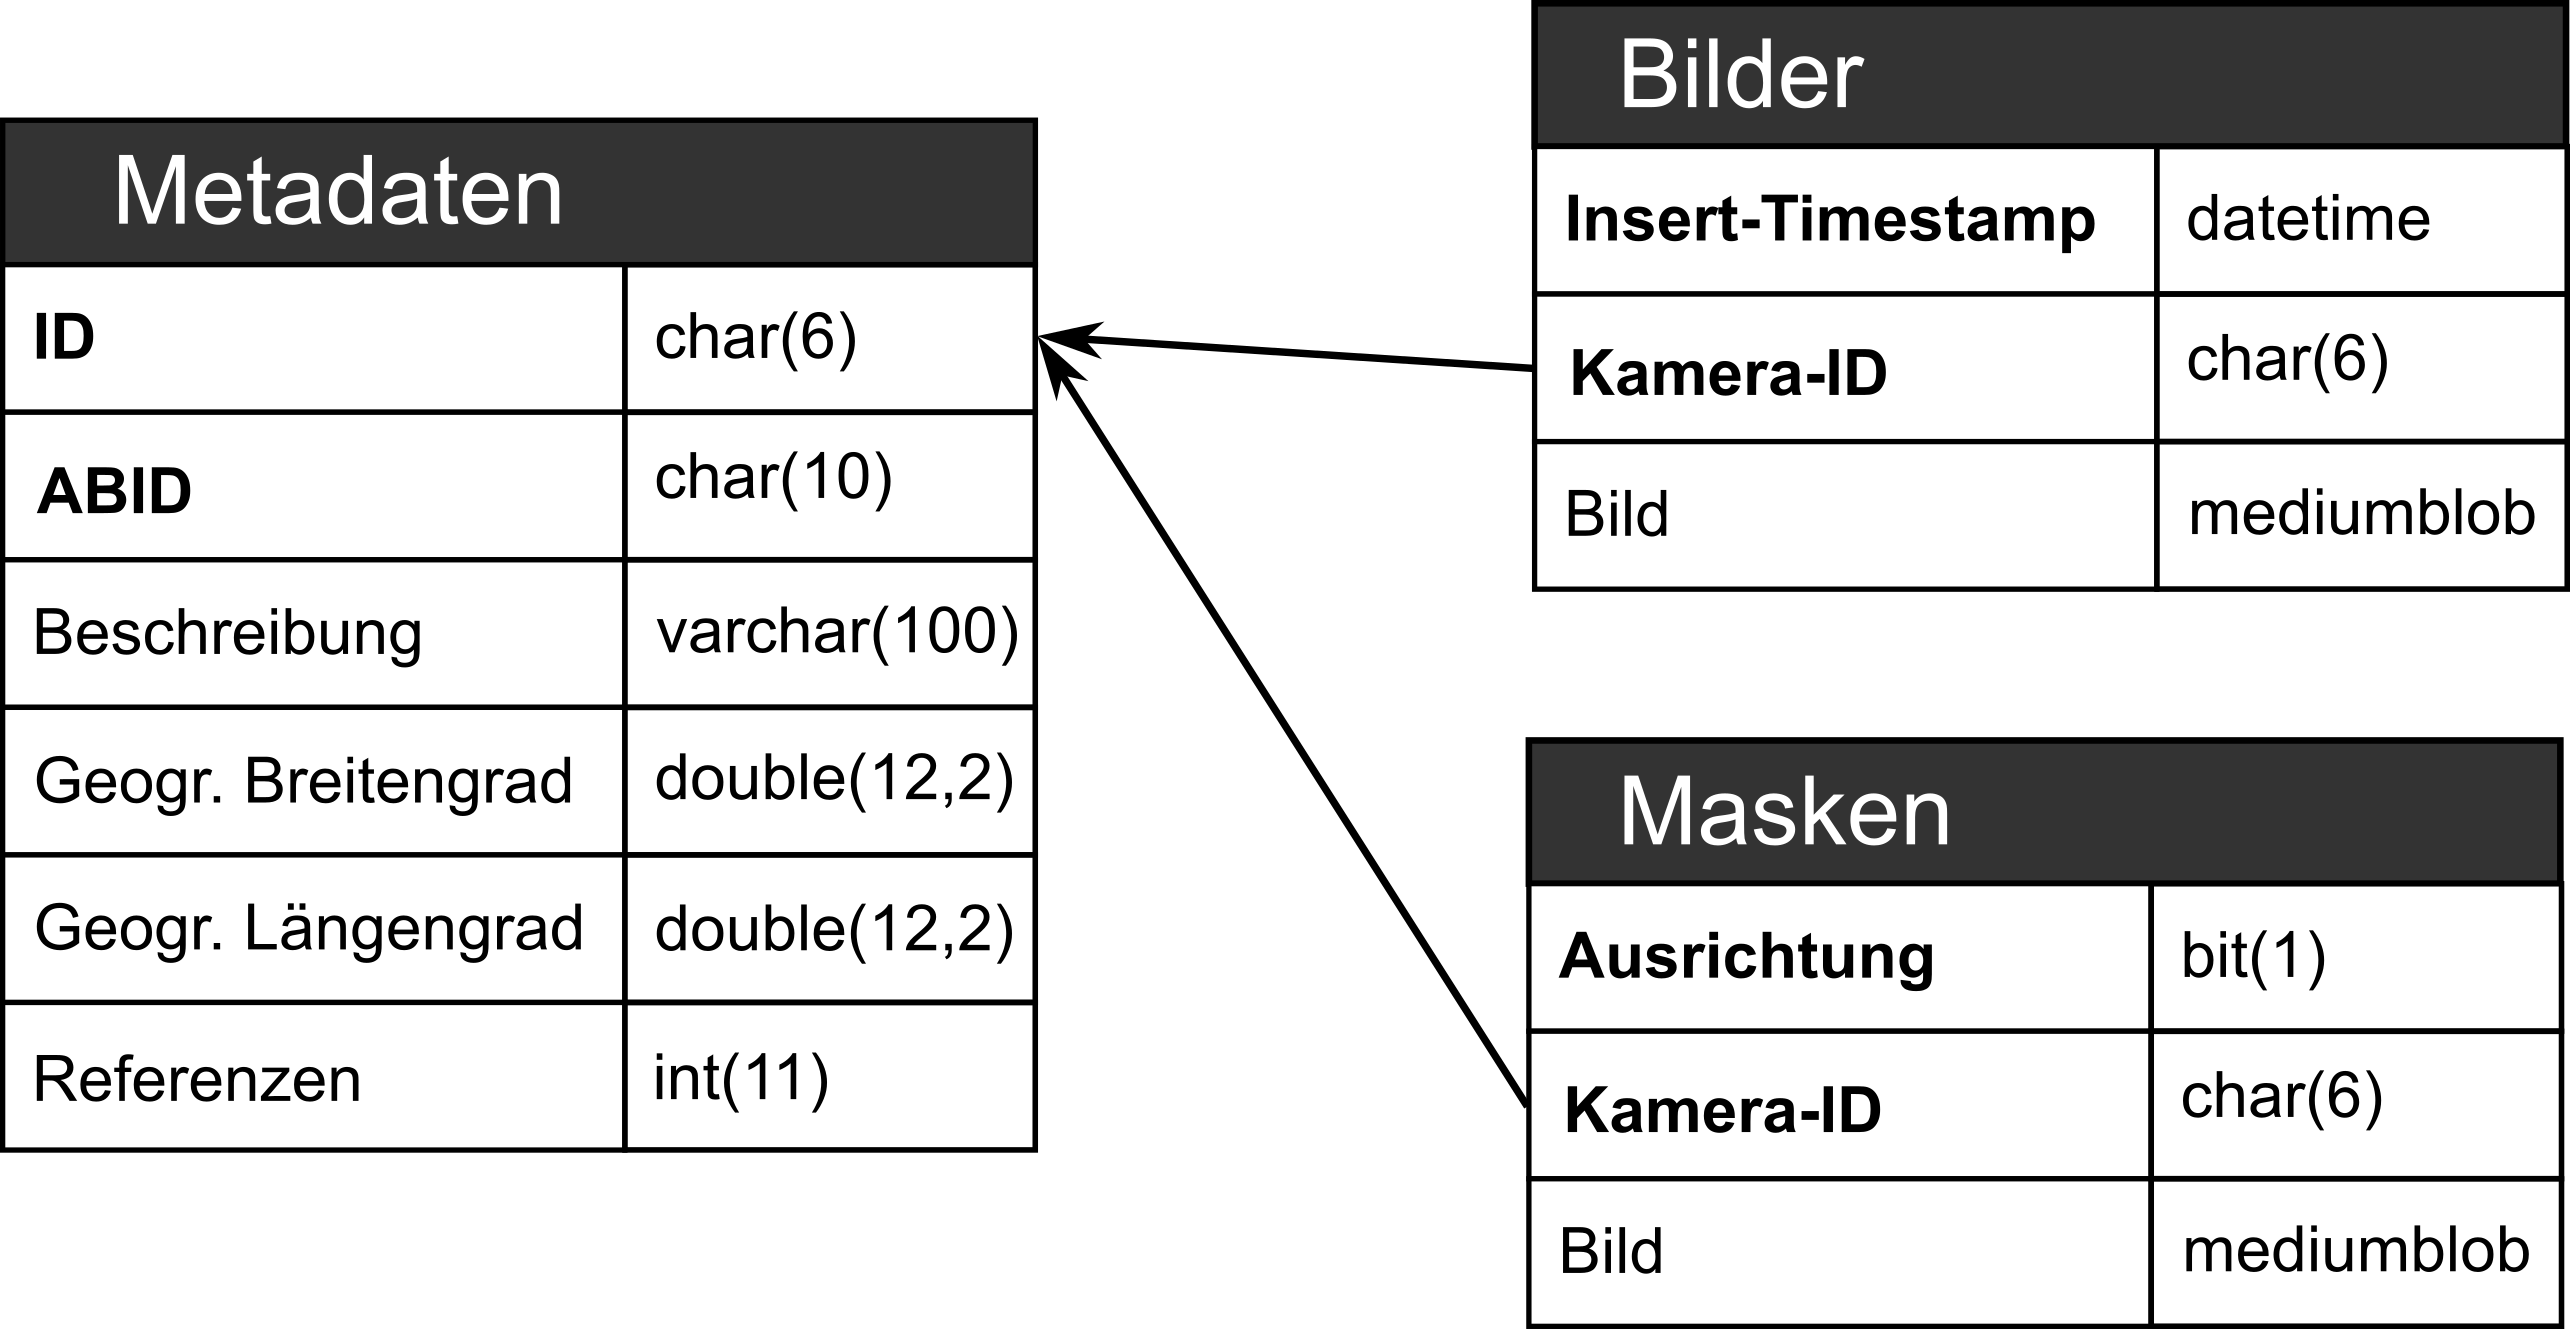
\includegraphics[width=15cm]{Bilder/db-schema} \\
 \caption{Datenbank Schema}
 \label{fig:dbschema}
\end{figure}

Damit PHP-Skripte auf die MySQL-Datenbank zugreifen können, gibt es zwei unterschiedliche APIs: Die "`PDO"'-API und die MySQLi-API. 
PDO steht dabei für PHP Data-Objects und bietet eine Unterstützung von mehreren Datenbank-Treibern. 
MySQLi, auch MySQL Improved Extension, begrenzt sich auf die Unterstützung von MySQL, bietet aber auch eine erweiterte Unterstützung neuer Funktionen von MySQL.
Da sich die Implementierung in dieser Arbeit auf eine MySQL-Unterstützung beschränkt wurde die letztere Programmierschnittstelle verwendet.

Damit die Datenbank mit Bildern, welche alle 30 Sekunden gespeichert werden, nicht vollläuft, gibt es einen Lösch-Mechanismus, der alte Datensätze automatisch aufräumt. 
Dieser ist in PHP implementiert und überprüft nach dem Einfügen eines Datensatzes, ob mehr als 10 Datensätze vorhanden sind.
Ist dies der Fall, werden die zehn jüngsten Datensätze behalten und der Rest gelöscht.
\newpage

\subsection{Datenbereitstellung}
Daten lassen sich vom Client, wie auf Abbildung~\ref{fig:serverarch} zu sehen, über HTTP-Anfragen an PHP-Skripte abrufen. Es gibt hierbei unterschiedliche Skripte, die für jeweils unterschiedliche Datensätze und Darstellungsarten verantwortlich sind:
\begin{itemize}
\item{kameras.php: Zuständig für das Abrufen aller erreichbaren Kameras mit deren Kennung}
\item{fetchmask.php: Zuständig für die Abfrage einer Maske für eine Verkehrskamera}
\item{fetcher.php: Zuständig für Abfragen von Bildern einer Verkehrskamera}
\end{itemize}
Das Skript "`kameras.php"' gibt bei einer Anfrage eine mit Leerzeichen separierte Liste aller Kennungen von Kameras zurück, welche eine Maske besitzen und einen Referenzzähler größer eins haben.
Der Referenzzähler ist dabei eine Hilfsvariable für das Backend, welche Kameras von Clients benötigt werden und daher die Bilder von ihnen heruntergeladen werden sollten.
Ein Client kann für eine oder mehrere Kameras den Referenzzähler inkrementieren, indem er das "`refcounter.php"' Skript mit den jeweiligen PHP-Skripten aufruft.

Das Skript "`fetchmask.php"' wird mit zwei Query-Paramteren aufgerufen: der Kamerakennung und der Ausrichtung, wobei Letzteres ein Binärwert ist. 
Es liefert, wie der Name bereits verrät, das PNG-Bild einer Maske für eine Kamera.

Das letzte Skript "`fetcher.php"' wird mit nur einem Query-Parameter für die Kamerakennung aufgerufen. 
Dieses Skript liefert einen Binärstrom aller gespeicherten Bilder einer Verkehrskamera, sowie den jeweiligen Zeitpunkt (in Unix-Zeit), wann dieses Bild auf dem SVZ-Server gespeichert wurde. 
Damit diese Daten korrekt vom Client gelesen werden können, werden die Daten in folgender Reihenfolge gesendet: Die Länge in Bytes des Zeitpunktes und des Bildes zusammen, der Zeitpunkt und Unix-Zeit und abschließend die Bytes des zusendenden JPEG-Bildes.
\newpage

\section{Client}
Der Client wird als eine Android Anwendung realisiert, die durch Kommunikation mit dem Backend und der Straßenverkehrszentrale das Problem der Stauerkennung so effizient und ressourcensparend wie möglich löst.
Durch das Verlagern der Berechnungen auf das mobile Endgerät, bleibt die Last des Backends gering und die Rechenleistung des Smartphones wird soweit ausgeschöpft, dass Berechnungen effizient, aber sparsam durchgeführt werden können.

\subsection{OpenCV}
Der Kern der Verarbeitung wird durch Algorithmen der OpenCV Bibliothek~\ref{sec:OpenCV} umgesetzt.
Da OpenCV primär als native Bibliothek zur Verfügung steht, bzw. die für Android nutzbare Java-Schnittstelle auf die native (in C++ geschriebene) Implementierung
zurückgreift, muss OpenCV für die jeweiligen Prozessoren der Android Geräte kompiliert werden, auf denen die Anwendung genutzt werden soll.

Eigentlich bietet OpenCV selbst bereits vorkompilierte Versionen der Bibliothek für alle gängigen CPUs und Android Geräte an, jedoch sind diese nicht vollständig.
OpenCV besteht nämlich eigentlich aus zwei teilen: der Kernbibliothek, also OpenCV selbst, aber zusätzlich noch einem Erweiterungsmodul namens {\em OpenCV-Contrib}.

Diese Erweiterung bietet zusätzlich zu den Standartalgorithmen des Kerns Erweiterungen und diverse andere Algorithmen an, welche Randprobleme abdecken und bei der regulären Nutzung der Bibliothek nicht benötigt werden.

Da für die Umsetzung der Anwendung ein spezieller Background-Subtraction Algorithmus benötigt wird, welcher nur in dem Erweiterungsmodul zur Verfügung steht, wird dieses hierfür benötigt.

Die vorkompilierte Version von OpenCV beinhaltet jedoch nicht die Erweiterungen, sodass diese nicht nutzbar ist.

Um die Bibliothek jedoch nicht selbst für jede Architektur kompilieren zu müssen, gibt es die Möglichkeit, die Bibliothek von dritten zu beziehen.
Entwickler unter dem Namen {\em QuickBird Studios} stellen auf der Plattform {\em GitHub} (\url{https://github.com/quickbirdstudios/opencv-android}) eine aktuelle Version von OpenCV mit allen Erweiterungen zur Verfügung, welche ganz einfach in die App eingebunden und genutzt werden kann.

\subsection{Backend Kommunikation}
\label{sec:BackendCom}
Da das Backend in PHP geschrieben ist, verläuft die Kommunikation über das HTTP-Protokoll an den entsprechenden Webserver.
Android stellt bei der Kommunikation über HTTP jedoch Ansprüche. Die Kommunikation muss auf dem Gerät asynchron geschehen. Das bedeutet, dass im Haupt-Thread,
also dem Programmfaden, welcher für das Darstellen der Oberfläche dient, keinerlei Netzwerkkommunikation geschehen darf. Dies könnte unter Umständen dazu führen, dass die Oberfläche einfriert, da, solange auf das Ende der Kommunikation gewartet wird, die Oberfläche nicht neu dargestellt werden kann.

Um sicherzustellen, dass Kommunikation asynchron verläuft, wird in der Klasse {\em Downloader} jegliche HTTP-Kommunikation gekapselt.
Hierzu wird innerhalb der Klasse ein neuer Thread gestartet, welcher für die Kommunikation zuständig ist. Vor dem Starten des Threads kann ein Callback-Objekt übergeben werden, welches nach Abschluss der Kommunikation die erhaltenen Daten übergeben bekommt und aufgerufen wird.

Ebenfalls stellt der {\em Downloader} sicher, dass pro Instanz der Klasse nur eine Anfrage zur gleichen Zeit abgehandelt werden darf. Dieses Verhalten ist für das spätere Laden der Bilder relevant.
Werden dennoch mehrere Verbindungen gleichzeitig benötigt, können einfach mehrere Instanzen der Klasse erstellt werden.

Für die Kommunikation mit dem Backend, ist der {\em BackendConnector} verantwortlich.
Über den Konstruktor kann die URL des Backends übergeben werden.
Mit Hilfe der {\em Downloader}-Klasse stellt dieser die Endpunkte des Backends als Methoden zur Verfügung:

\begin{itemize}
\item{{\em cameras}: liefert eine Liste aller Unterstützten Kameras zurück}
\item{{\em fetch}: liefert entweder alle gespeicherten Bilder einer Kamera, oder alle Bilder jünger als ein gewünschter Zeitpunkt}
\item{{\em mask}: liefert die Maske für eine Kamera in eine gewünschte Fahrtrichtung}
\end{itemize}

Die Ergebnisse aller Anfragen liegen jedoch im Rohformat als Byte-Array vor. Um die Ergebnisse also nutzen zu können, ist also eine weitere Verarbeitung der Daten in einem späteren Schritt nötig.

\subsection{Geolokalisierung}
Um gezielt Kameras abzufragen und auszuwerten, ist es sinnvoll nur diese auszuwerten, die in unmittelbarer Nähe des Nutzers sind und ebenfalls Relevanz für die Fahrt haben. Hierfür muss demnach die Position des Nutzers ermittelt und ausgewertet werden.

Heutige Smartphones besitzen in der Regel ein GPS-Modul, mit welchem sich die Position bestimmen lässt.
Bevor man jedoch die Möglichkeit hat, mit dem Modul kommunizieren zu können, muss eine Anwendung die erforderlichen Berechtigungen einfordern.
Dafür muss zunächst in der Manifestdatei der Android-Anwendung die Berechtigung {\em android.permission.ACCESS\_FINE\_LOCATION} hinzugefügt werden.
Bei neueren Android-Versionen reicht dies allein jedoch nicht mehr aus. Zusätzlich dazu muss der Nutzer explizit bestätigen, dass die Anwendung Zugriff auf den Standort erhält.

Durch Übergabe des Wertes {\em Manifest.permission.ACCESS\_FINE\_LOCATION} an die Funktion {\em requestPermission} der {\em Activity}-Klasse, die den Einstiegspunkt der Android-Anwendung bietet, wird dem Nutzer ein Dialog angezeigt, durch welchen er Zugriff erteilen oder verweigern kann.


Sind alle Berechtigungen erteilt, so kann die App den Standort abfragen.
Hierfür ist in der App die Klasse {\em GlobalPositionManager} verantwortlich. Diese kapselt die Interaktion mit dem GPS-Modul und kann über an einen übergeben Callback Standortänderungen regelmäßig nach außen kommunizieren.
Hierzu wird zunächst beim {\em LocationManager}, dem System Dienst für die Standortverwaltung des Gerätes, die Lokalisierung angefragt, was dafür sorgt, dass alle 10 Sekunden der aktuelle Standort and den {\em GlobalPositionManager} übergeben wird. Dieser kann anschließend an den Callback übergeben werden und für die weitere Verarbeitung genutzt werden.

\subsection{Richtungsfestellung}
Hat man nun die Position zur Hand, so ist als Nächstes relevant zu wissen, wohin gefahren wird, um die zu analysierende Straßenseite zu erkennen.
Hierfür gibt es diverse Ansätze, um das Problem zu lösen.

Beispielsweise stellt Google einen Dienst zur Verfügung, über den bei Übergabe von verschiedenen Positionen die befahrene Straße und Richtung erkannt werden kann. Dieser ist jedoch kostenpflichtig und deshalb nicht geeignet.

Um auch hier den Fokus auf Ressourcensparsamkeit nicht zu verlieren, wurde ein sehr einfacher, jedoch nicht generischer Ansatz gewählt.
Da die Anwendung primär für eine Nutzung auf der A5 gedacht ist, ist das Ziel zunächst nur die Fahrtrichtung auf der A5 zu erkennen.
Auf anderen Autobahnen kann daher nicht ohne Weiteres erkannt werden, auf welcher Straßenseite gefahren wird.

Die A5 erstreckt sich von Niederaula, nördlich von Frankfurt am Main bis nach Weil am Rhein, kurz vor vor der Schweizer Grenze. Grob gesehen kann man sagen sie erstreckt sich von Frankfurt nach Basel.

Um nun die Fahrtrichtung zu erkennen, können die Standorte über die Zeit protokolliert und kumuliert werden, um daraus einen Richtungsvektor zu bilden.
Dieser kann genutzt werden, um abzuschätzen, ob der sich Nutzer Frankfurt oder Basel nähert.

Dazu werden die vom {\em GlobalPositionManager} erfassten Positionen durch die Klasse {\em PositionHistory} protokolliert.
Über die bereitgestellten Methoden {\em getStart} und {\em getEnd} werden die Positionen so aufsummiert, dass Startpunkt und Endpunkt ausgelesen werden können.

Anschließend ermittelt die Klasse {\em DirectionCalculator} die euklidische Norm zwischen sowohl Frankfurt, als auch Basel und den Start- und Endpunkten.
Diese vernachlässigt zwar die Krümmung der Erdoberfläche und jegliche Höhenunterschiede, ist aber für solch kurze Distanzen völlig ausreichend.

Ist der Startpunkt nun weiter entfernt von Frankfurt als der Endpunkt, so bewegt sich der Nutzer nach Frankfurt, ansonsten in Richtung Basel.

Anfangs ist das Feststellen der Richtung noch recht ungenau. Je mehr Positionen jedoch über die Zeit protokolliert werden, desto genauer wird die Ermittlung der Fahrtrichtung.

Obwohl diese Form der Richtungsfeststellung nur auf der A5 funktioniert, ist die Berechnung sehr effizient und akkurat, da nur wenige einfache Rechenschritte benötigt werden, um somit der Ressourcensparsamkeit gerecht zu werden.

\subsection{Verkehrskameras laden}
Bevor die Informationen zu den Verkehrskameras von der Straßenverkehrszentrale geladen werden können, muss zunächst geprüft werden, welche Kameras das Backend unterstützt.

Hierfür kann über die Klasse {\em AvailableCamerasLoader}, wie im Abschnitt~\ref{sec:BackendCom} beschrieben, über den {\em BackendConnector} mit der Methode {\em cameras} die Liste der unterstützten Kameras abgerufen werden.
Die IDs der Kameras zeilenweise zurückgeliefert. Der {\em AvailableCamerasLoader} verarbeitet die Zeilen anschließend, sodass eine Liste der verfügbaren Kamera IDs zur Verfügung steht.

Zusätzlich dazu werden noch die detaillierten Kamerainformationen der Straßenverkehrszentrale benötigt. Dafür kann über den {\em CameraLoader}, wie im Abschnitt~\ref{sec:AnaCam}, die Liste der Kameras mit dem {\em Downloader} empfangen werden und und verarbeitet werden. Hierfür wird das Tabellenformat aufgeschlüsselt und die benötigten Werte wie ID, Name, Beschreibung und Standort der Kamera in einem {\em Camera}-Modell abgelegt werden.

Da der Standort jedoch ein unterschiedliches Koordinatensystem verwendet, muss dieser jedoch noch konvertiert werden. Hierfür kann über die Bibliothek Proj4J~\cite{proj4j} eine Konvertierung durchgeführt werden.

Diese empfangene Liste wird nun anhand den vom Backend unterstützten Kameras gefiltert, sodass nur noch diese verfügbar sind, mit denen auch gearbeitet werden kann.

Schließlich wird beim Aktualisieren der Position des Nutzers, bzw. auch der Fahrtrichtung, geprüft, welche Kameras für die Weiterfahrt relevant sind. Das bedeutet Kameras die nicht auf der Strecke liegen, werden erst gar nicht benötigt. Liegen Kameras zwar auf der Strecke, aber hinter dem Nutzer, also ist der Nutzer bereits an ihnen vorbei gefahren, so sind diese ebenfalls nicht mehr relevant. Lediglich die Kameras, die vor dem Nutzer auf der Strecke sind, werden für die Stauanalyse benötigt. 
Es wird also nach jeder Positionsänderung geprüft, welche Kameras relevant sind. Diese werden dann markiert, sodass die spätere Bildanalyse weiß, welche Kameras analysiert werden sollen.

\subsection{Bilder laden}
Das Laden der Bilder gliedert sich in 3 Hierarchiestufen.
Auf der untersten Ebene kann über die {\em fetch}-Methode des {\em BackendConnectors} ein Binärstream an Bilddaten vom Backend für eine Kamera geladen werden.
Da das Backend innerhalb dieses Streams alle Bilder liefert, die es zwischen gepuffert hat, müssen diese zunächst voneinander getrennt werden.

Eine Hierarchieebene darüber regelt der {\em MultiImageLoader} die Verarbeitung.
Nach Erhalt der Rohdaten des Backends wird der Binärstrom aufgespalten.
Jedes Teilbild innerhalb des Stroms hat einen Kopf, welcher aus 4 Bytes für die Länge des Bildes und 8 Bytes für den Aufnahmezeitpunkt des Bildes besteht.
Nach den Kopfdaten folgt das eigentliche Bild. Der gesamte Strom besteht nun einer Folge von Kopf und Bild. Wobei zu beachten gilt, dass die Bytereihenfolge des Kopfes {\em Little-Endian} ist, und nicht {\em Big-Endian} wie auf den meisten Android Geräten verwendet.

Es wird also die Länge des Bildes gelesen und konvertiert, danach der Zeitpunkt gelesen und konvertiert und anschließend das Bild über die vorher eingelesene Länge extrahiert. Dieser Vorgang wiederholt sich solange, bis idealerweise keine Bytes mehr im Strom sind, oder im Fehlerfall die aus dem Kopf entnommene Länge des Bildes länger ist, als übrige Bytes im Strom vorhanden sind.

Das Backend liefert standardmäßig jedoch alle Bilder für eine Kamera die es zwischengespeichert hat. Um also nicht bei jeder Anfrage alle Bilder alten Bilder erneut empfangen und verarbeiten zu müssen, wird in der obersten Hierarchiestufe vom {\em CameraImageFetcher} das Strukturierte laden der Bilder koordiniert.

Für jede der relevanten Kameras existiert eine Instanz, die von außerhalb alle 29 Sekunden aufgefordert wird neue Bilder abzurufen. Das sorgt, dafür, dass mindestens 2 mal innerhalb der Aktualisierungsperiode des Straßenverkehrszentrums auf neue Bilder geprüft wird, um möglichst schnell auf Stau reagieren zu können und die Latenz des Ladens und Verarbeitens der Bilder zu kompensieren.

Die vom {\em MultiImageLoader} empfangenen Bilder werden also zwischengespeichert. Bei einem neuen Abfrageintervall kann über das Durchreichen des Zeitstempels des letzten empfangenen Bildes an den {\em BackendConnector} das Backend dazu instruiert werden, lediglich die Bilder zu senden, die jünger als der besagte Zeitstempel sind.

\subsection{Bilder verarbeiten}
Die Verarbeitung der Bilder wird von der Klasse {\em EvaluationExecutor} verwaltet.
Diese hört sowohl auf Änderungen der relevanten Kameras, als auch auf Änderungen der Fahrtrichtung.

Für jede Kamera wird zunächst eine passende Maske für die entsprechende Fahrtrichtung vom Backend geladen.
Hierfür kann über den {\em BackendConnector} mit der {\em mask} die entsprechende Maske angefordert werden.

Diese dient bei der Verarbeitung dazu, die irrelevanten Teile des Bildes, wie beispielsweise Fahrbahnränder oder die Gegenfahrbahn zu verdecken, um das Ergebnis zu optimieren.

Ebenfalls wird der {\em EvaluationExecutor} benachrichtigt, sobald neue Bilder vom Backend empfangen wurden.
Um diese nun zu verarbeiten, gibt es für jede Kamera eine Instanz der {\em ImageEvaluator}-Klasse, welche für die eigentliche Verarbeitung der empfangenen Bilder zuständig ist.

Die eigentliche Verarbeitung der Bilder gliedert sich in 5 Teilschritte.

\begin{figure}[ht]
   \centering
     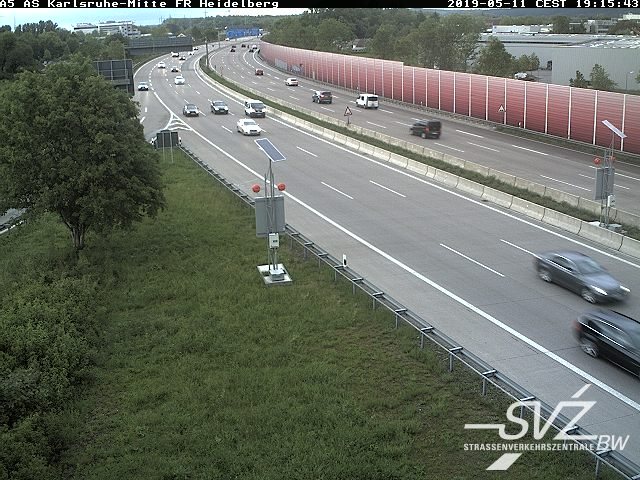
\includegraphics[width=7cm]{Bilder/process/1} \\
 \caption{Zu verarbeitendes Beispielbild}
\end{figure}

\paragraph*{Vorverarbeitung}
Bei der Vorverarbeitung wird ein empfangenes Bild so aufbereitet, dass die nachfolgende Verarbeitung bessere Ergebnisse liefert.

Hierfür wird das Bild zunächst gemittelt, um mögliche Rauschanteile zu reduzieren.
Mit der von OpenCV bereitgestellten Methode {\em Imgproc.blur} lässt sich ein Bild weichzeichnen.

Anschließend wird auf das weichgezeichnete Bild die geladene Maske aufgetragen.

Wichtig ist, dass die Maske nach der Mittelung aufgetragen wird und nicht vorher, da sonst die Maske negative Auswirkungen auf die Qualität des gemittelten Bildes haben kann.

\begin{figure}[ht]
   \centering
     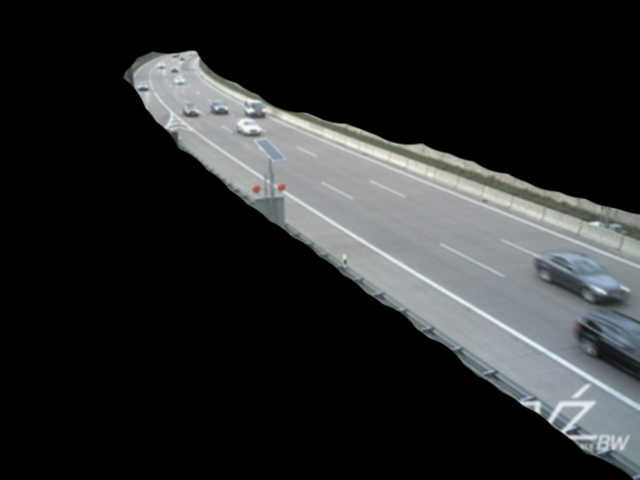
\includegraphics[width=7cm]{Bilder/process/2} \\
 \caption{Ergebnis nach der Vorverarbeitung}
\end{figure}

\paragraph*{Verarbeitung}
Bei der Verarbeitung gilt es die Autos vom Hintergrund zu trennen. Dazu wird der von OpenCV bereitgestellte Background-Subtractor namens {\em MOG} verwendet.
Dieser liefert auf ein übergebenes Bild ein Binärbild zurück, bei welchem schwarze Pixel den Hintergrund symbolisieren und weiße Pixel die Objekte im Vordergrund, welche idealerweise alles Autos sein sollten.

Damit dieser Algorithmus jedoch verlässliche Ergebnisse liefert, muss dieser zunächst trainiert werden. 
Aus diesem Grund liefert das Backend nicht nur das aktuellste Bild, sondern eine Sequenz von zeitlich eng beieinanderliegenden Bildern, mit welchen der Background-Subtractor trainiert werden kann. 

\begin{figure}[ht]
   \centering
     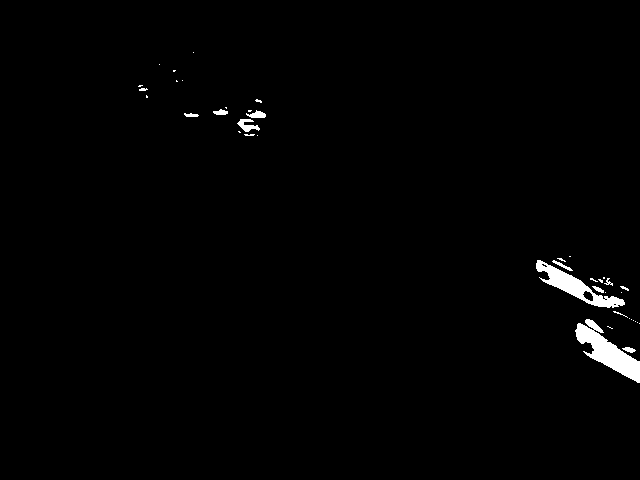
\includegraphics[width=7cm]{Bilder/process/3} \\
 \caption{Ergebnis nach der Verarbeitung}
\end{figure}

\paragraph*{Nachbearbeitung}
Dieser Schritt und alle Nachfolgenden, sind lediglich für die Bilder relevant, die auch ausgewertet werden sollen, und nicht nur zum Trainieren des Background-Subtractors dienen.

Bei der Nachbearbeitung wird versucht jegliche Artefakte oder Ungenauigkeiten, die bei der Verarbeitung des Bildes entstanden sind, zu entfernen.
Beispielsweise werden Autos nicht immer als geschlossene Konturen dargestellt oder es entstehen Verbindungen zwischen Autos und größeren Transportern, die parallel zueinander fahren, wodurch diese als eine einzige Kontur erkannt werden könnten. Darüber hinaus kann es vorkommen, dass vereinzelt weiße Pixel auftauchen, welche vermutlich durch Rauschen, Schatten, oder andere Bedingungen fälschlicherweise als Objekte eingestuft wurden.

Um diese Artefakte zu entfernen, kann eine Kombination von morphologischen Operatoren angewendet werden.

Zunächst wird versucht über {\em Closing} die Konturen der Autos zu schließen, bzw. getrennte Teile eines Autos zu vereinen.
Anschließend sollen über {\em Opening} kleine weiße Pixel und alleinstehende Artefakte entfernt werden.

Zuletzt wird mit einer {\em Dilatation} versucht die Konturen der Autos zu verkleinern, um mögliche Verbindungen oder Fehlinterpretationen von Verbindungen zu Transportern zu verhindern.

\begin{figure}[ht]
   \centering
     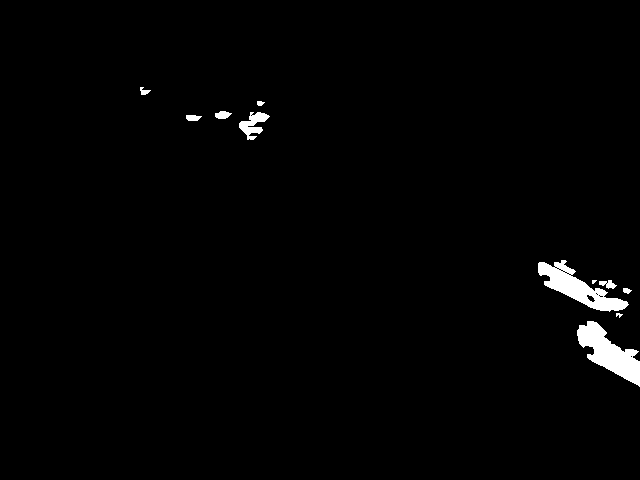
\includegraphics[width=7cm]{Bilder/process/4} \\
 \caption{Ergebnis nach der Nachbearbeitung}
\end{figure}

\paragraph*{Analyse}
Bei der Analyse wird versucht Konturen zu erkennen, und diese zu vereinen.
Über die Methode {\em Imgproc.findContours} von OpenCV, lassen sich Konturzüge aus einem Binärbild auslesen.
Zur effizienteren Verarbeitung wird der Polygonkonturzug jedoch auf einfache Rechtecke reduziert, indem der Minimale und Maximale Punkt der Kontur in sowohl X-, als auch Y-Richtung zur Bildung des Rechtecks gewählt wird, wodurch eine Hülle um den Zug gebildet wird.

Da es trotz Nachbearbeitung vorkommen kann, dass Konturen innerhalb von Konturen erkannt werden, oder einige sich überlappen, wird versucht Konturen zu vereinen.

Dabei werden Konturen innerhalb einer anderen Kontur vollständig entfernt. Überlappen sich zwei Konturen, so werden diese zu einer großen Kontur vereint.

Dieser Prozess wird solange iterativ durchgeführt, bis sich keine Kontur mehr verändert.

\begin{figure}[ht]
   \centering
     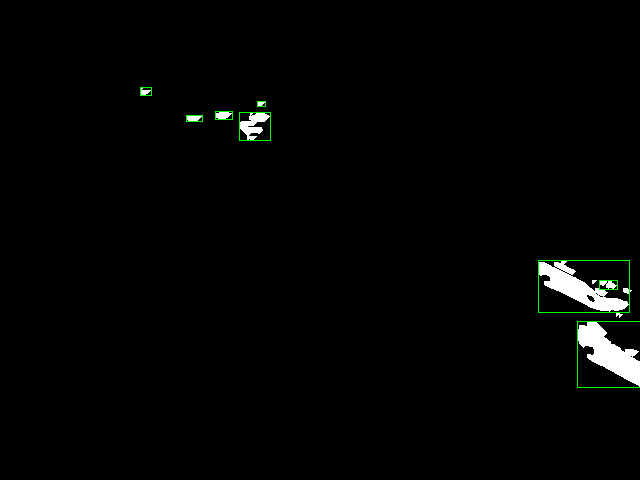
\includegraphics[width=7cm]{Bilder/process/5_1}
		 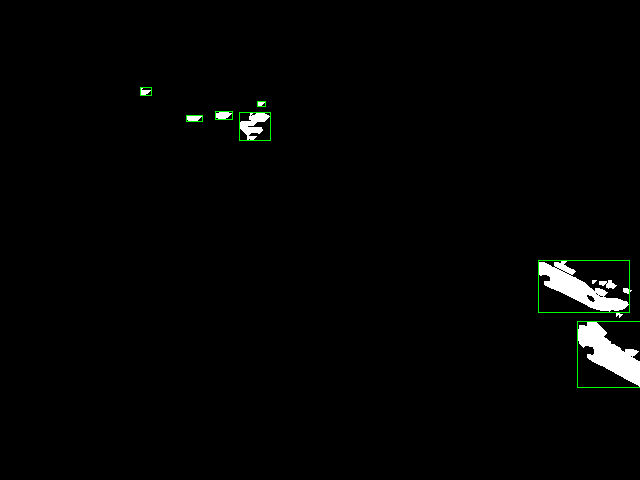
\includegraphics[width=7cm]{Bilder/process/5_2} \\
 \caption{Konturen erkennen und schließen}
\end{figure}

\paragraph*{Klassifikation}
Bei der Klassifikation wird nun versucht anhand der Konturen eine Aussage über die Verkehrssituation zu treffen.
Hierbei wird jede erkannte Kontur als Auto betrachtet.
Um nun einzuschätzen, ob Stau ist oder nicht, wird der Anzahl der Konturen mit einem vordefinierten Limit für die jeweilige Kamera verglichen. Hierbei wird jedoch nicht wie bei einem Thresholding-Verfahren ab überschreiten der Grenze Stau erkannt, sondern versucht ab einer Anzahl an Konturen größer als die Hälfte des Limits eine prozentuale Aussage über die Stauwahrscheinlichkeit zu treffen.

\begin{figure}[ht]
   \centering
     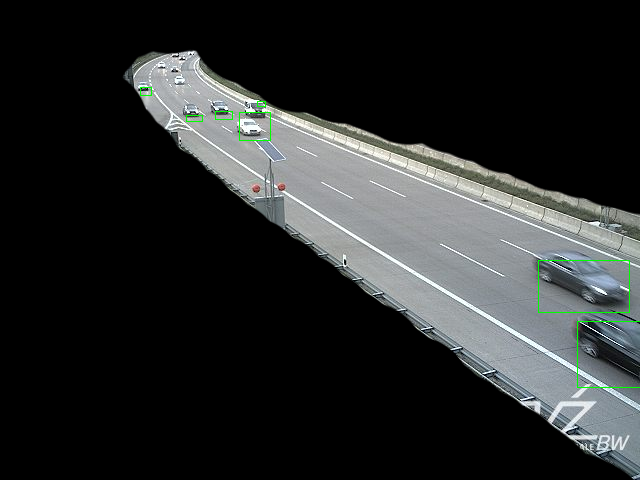
\includegraphics[width=7cm]{Bilder/process/6} \\
 \caption{Vollständig verarbeitetes Bild}
\end{figure}

Liegt das Limit einer Kamera bei beispielsweise 40 Autos und es wurden 30 Autos erkannt, so ist die Hälfte des Limits (20) überschritten. Es wird also versucht eine Aussage über die Wahrscheinlichkeit zu treffen. Da 30 Autos genau in der Mitte zwischen der Hälfte und dem gesamten Limit liegen, wird eine Stauwahrscheinlichkeit von 50\% angenommen.

\subsection{Bluetooth}
Ein Wunsch war es, dass sich die Anwendung automatisch startet, sobald mit dem Auto gefahren wird.
Hierfür muss demnach erkannt werden, wann ein Nutzer im Auto sitzt.

Der beste Ansatz hierfür ist es, zu erkennen, wann das Handy eine Bluetooth-Verbindung zur Freisprechanlage des Autos aufgenommen hat, um daraufhin die Anwendung zu starten.

Diese Aufgabe übernimmt der {\em BluetoothDeviceChecker}. Zunächst ermöglicht er die mit dem Gerät verbundenen Bluetooth-Geräte auszulesen.

Darüber hinaus können Bluetooth-Geräte gespeichert, ausgelesen und gelöscht werden, die einen Start der App bei einer Verbindung auslösen sollen.
Dazu werden die MAC Adressen (Media-Access-Control) der Geräte als JSON codierte Liste auf dem Speicher des Smartphones abgelegt.

Ebenfalls gibt es die Möglichkeit lediglich zu prüfen, ob das Smartphone zurzeit mit einem Gerät gekoppelt ist, welches den Start der App auslösen soll.

Um nun vom System benachrichtigt zu werden, wenn ein neues Bluetooth-Gerät verbunden wurde, ohne, dass die Anwendung bereits läuft, gibt es in Android die Möglichkeit einen Service zu registrieren.
Dieser kann dem System mitteilen, welche Ereignisse für ihn relevant sind, sodass das System den Service benachrichtigt, sobald ein solches Ereignis eingetreten ist.

Für den Start der Stauanalyse wird also ein Service mit dem namen {\em BluetoothService} registriert, welcher auf Events, bzw. Intents des Typs {\em android.bluetooth.device.action.ACL\_CONNECTED} hören. Dieses Ereignis wird ausgelöst, wenn eine neue Bluetooth-Verbindung aufgebaut wurde.

Innerhalb des {\em BluetoothService} kann nun bei eintreffen der Benachrichtigung mit dem {\em BluetoothDeviceChecker} geprüft werden, ob das Gerät den Start der App auslösen soll. Ist das der Fall, so kann zum Start der Anwendung ein neuer Intent ausgelöst werden. Über diesen Intent kann dem System mitgeteilt werden, dass die Anwendung gestartet werden soll, falls sie nicht bereits gestartet wurde.

\subsection{Benutzeroberfläche}
Obwohl die Anwendung hauptsächlich akustisch mit dem Nutzer kommuniziert, wird eine grafische Oberfläche benötigt.
Dennoch ist das Aussehen und die Funktionalität der Oberfläche sehr schlicht, da diese nur eine sekundäre Rolle spielt.

Untergliedert wird die Anwendung dabei in 3 verschiedene Tabs, durch die navigiert werden kann:

\paragraph*{Map}
Die erste Ansicht ist eine Landkarte, die auf dem freien Kartendienst OpenStreetMaps basiert. % Vlt. Referenz?
Diese soll sowohl den Standort des Nutzers anzeigen, als auch alle geladenen Kameras anzeigen, sodass der Nutzer eine Übersicht hat,
welche Kameras es gibt, und wo sie positioniert sind.

\begin{figure}[ht]
   \centering
     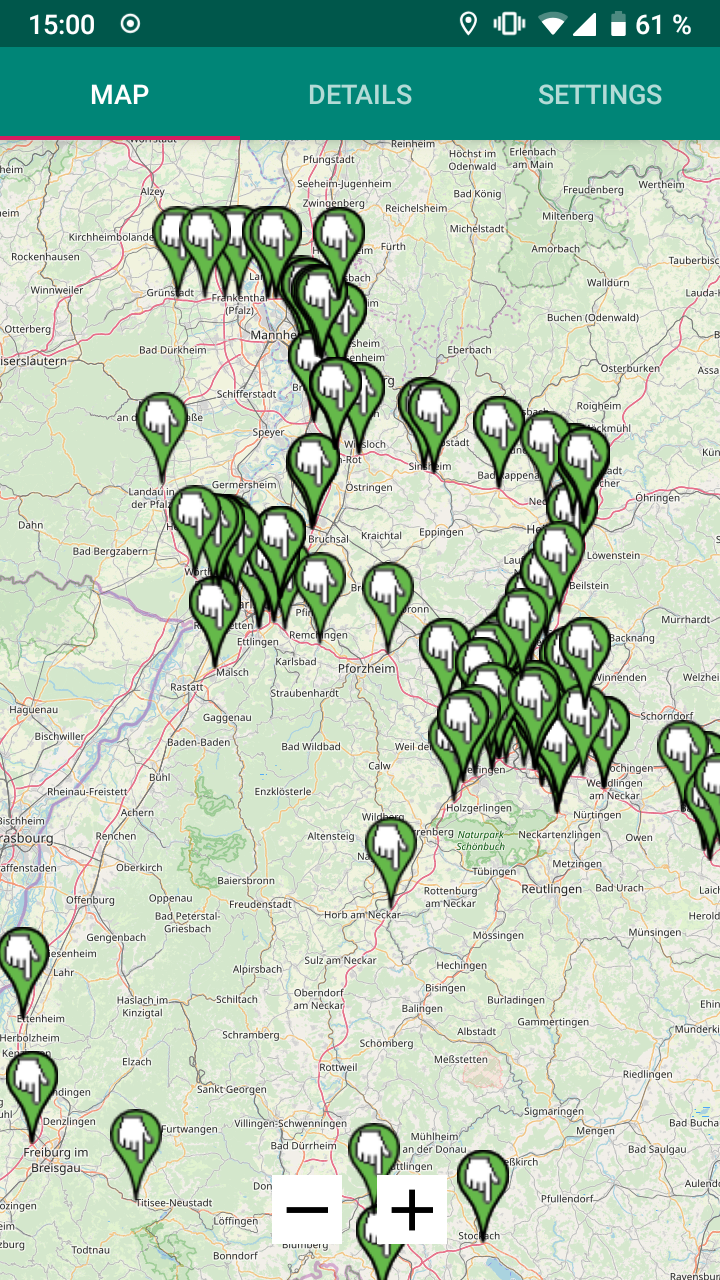
\includegraphics[width=5cm]{Bilder/app-map} \\
 \caption{Kartenansicht der Anwendung}
\end{figure}

\paragraph*{Details}
Die Detailseite zeigt dem Nutzer Details zum Analyseprozess.
Zum einen lässt sich in einer Debugansicht sehen, welche Schritte des Analyseprozesses durchlaufen wurden (beispielsweise Feststellung des Standorts, Feststellung der Richtung, Laden der Kameras, Analyse der Bilder, usw.).
Darüber hinaus hat der Nutzer auch die Möglichkeit zu jeder analysierten Kamera das zuletzt ausgewertete Bild zu sehen, auf welchem die erkannten Autos markiert wurden. Anhand dessen kann der Nutzer dann selbst noch einmal einschätzen, ob die Aussage der Anwendung zur Verkehrslage korrekt ist, oder nicht.

\begin{figure}[ht]
   \centering
     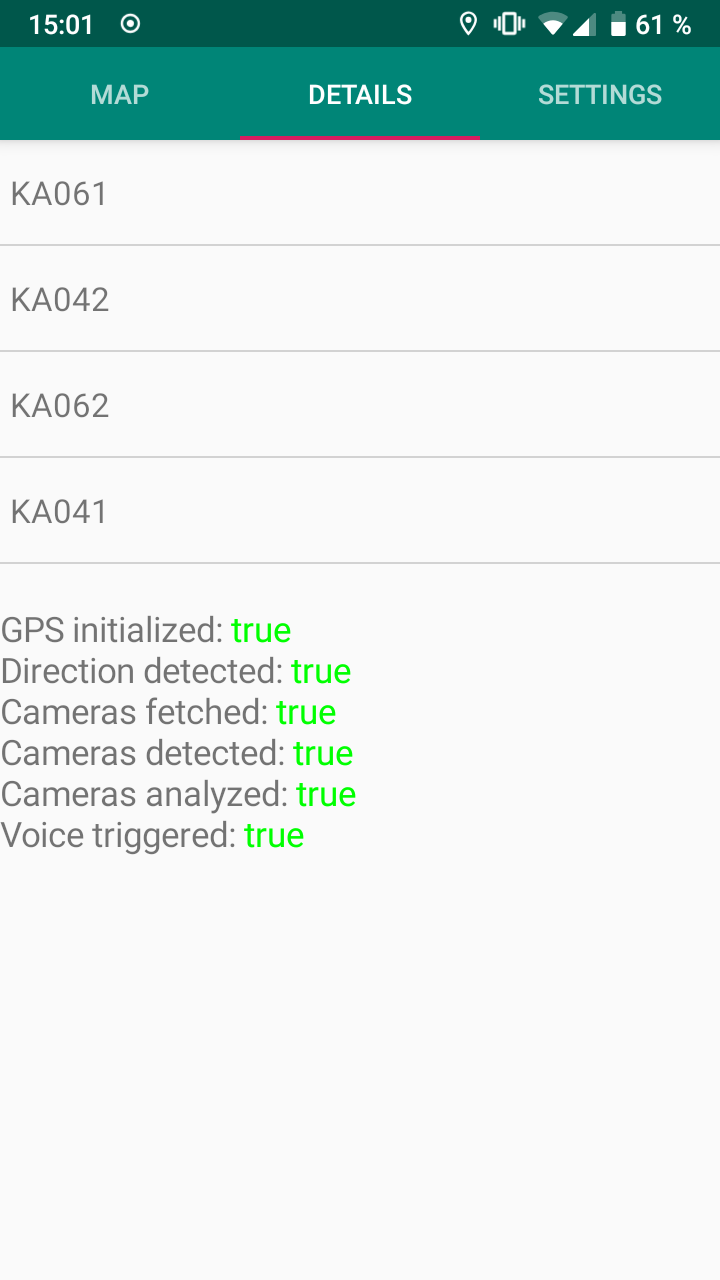
\includegraphics[width=5cm]{Bilder/app-details}
     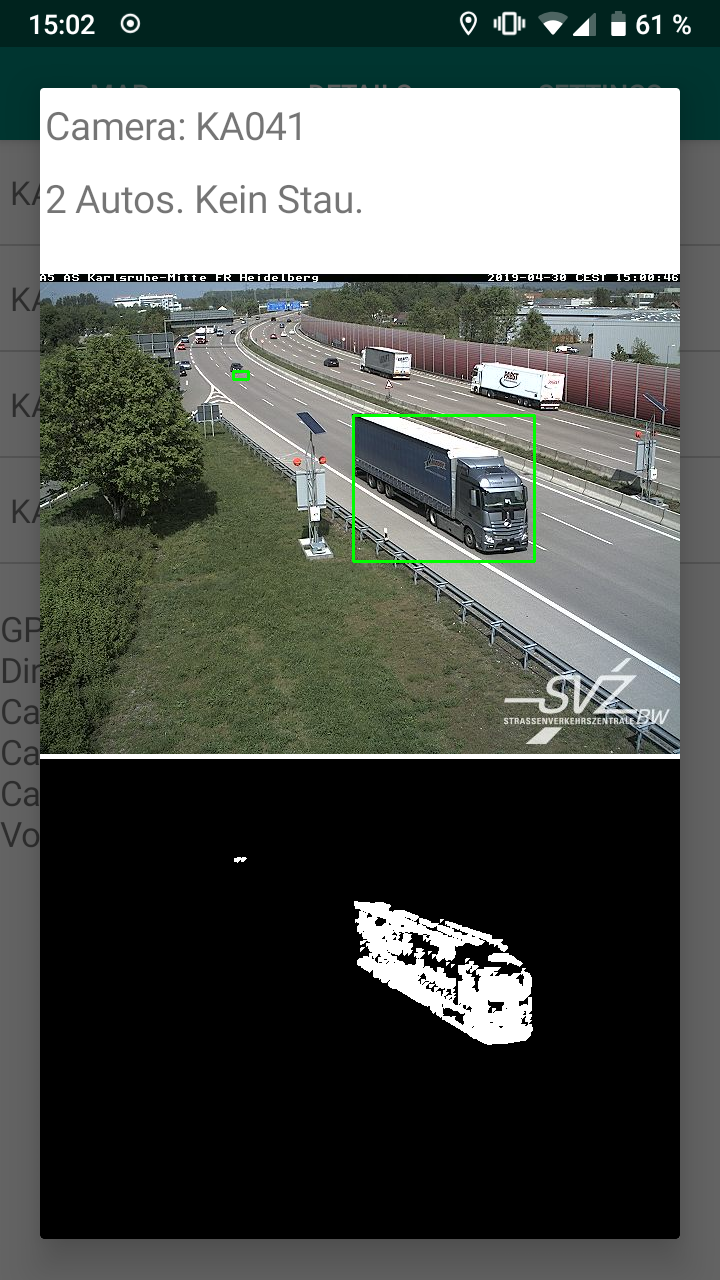
\includegraphics[width=5cm]{Bilder/app-details-cam} \\
 \caption{Detailansicht der Anwendung}
\end{figure}

\paragraph*{Settings}
Die Einstellungsseite dient zur Konfiguration der Bluetooth-Geräte.
Hierbei sieht der Nutzer eine Liste aller mit dem Handy gepaarten Geräte und hat durch Anklicken dieser die Möglichkeit das Gerät zu speichern, sodass die Kupplung den Start der App auslöst.

Ebenfalls gibt es eine zweite Liste, über die der Nutzer Geräte wieder entfernen kann, sodass diese den Start der App nicht mehr auslösen.

\begin{figure}[ht]
   \centering
     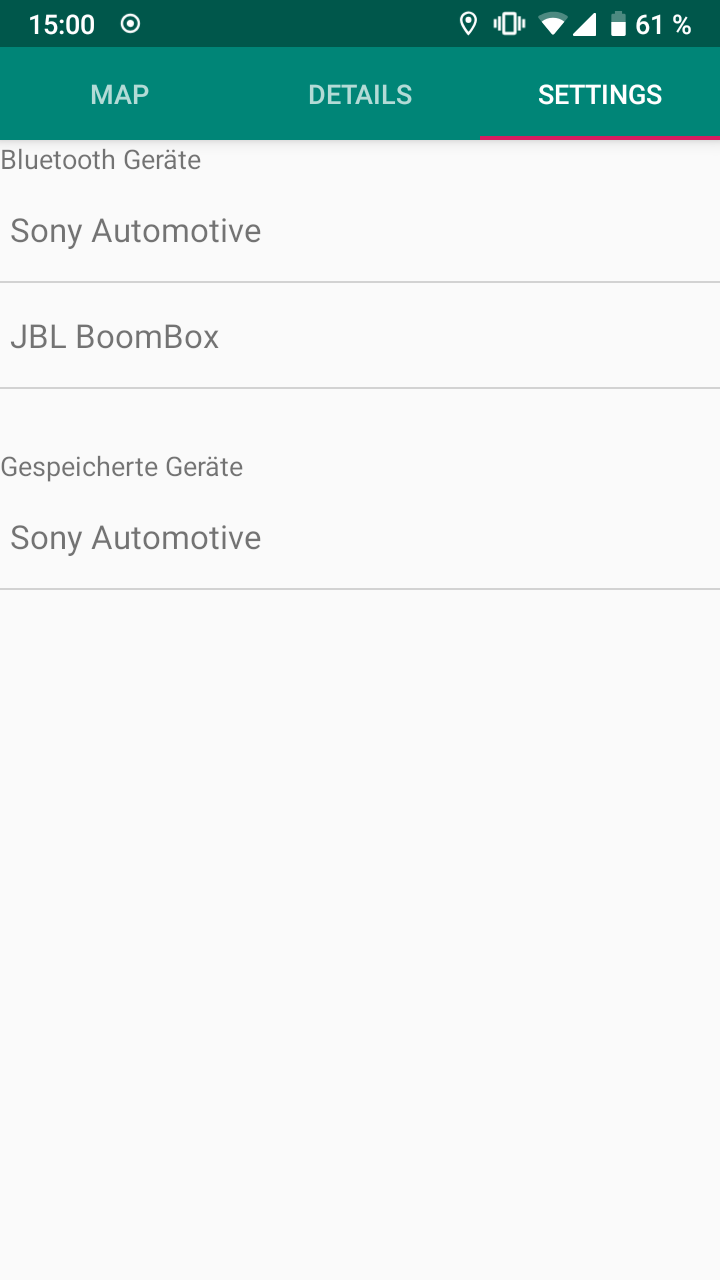
\includegraphics[width=5cm]{Bilder/app-settings} \\
 \caption{Einstellungen der Anwendung}
\end{figure}

\subsection{Stauansage}
Die Ansage des Staus untergliedert sich technisch in zwei Teile. Im ersten Teil wird die grundsätzliche Textansage realisiert und zusätzlich die Integration einer Bluetooth-Freisprechanlage ermöglicht.
Der zweite Teil übernimmt die kontextbezogene Ansage des Verkehrszustandes.

Um überhaupt Informationen per Sprachausgabe vermitteln zu können, wird die interne Android {\em Text-To-Speech}-API verwendet.
Die Klasse {\em Speaker} übernimmt die Kapselung der Schnittstelle.

Nach außen exponiert die Klasse lediglich eine Methode {\em speak}, die bei Übergabe von Text, eine Sprachausgabe auslösen soll.

Da die interne {\em Text-To-Speech}-API eine unbestimmte Zeit zur Initialisierung benötigt, können Nachrichten nicht direkt ausgegeben werden, sondern werden zunächst in einer Warteschlange gesammelt, bis die Initialisierung abgeschlossen ist.

Um die Sprachausgabe auch über eine Freisprechanlage in einem Auto zu ermöglichen, wird, vor der Übergabe einer Nachricht an das System, geprüft, ob das Gerät mit einem Auto gekoppelt ist. Hierzu kann der {\em BluetootDeviceChecker} genutzt werden.

Ist ein kompatibles Gerät gekoppelt, übermittelt der {\em Speaker} an das System, dass der Bluetooth-SCO-Modus für die Audiowiedergabe aktiviert werden soll. Das sorgt dafür, dass Töne nicht mehr über reguläre Lautsprecher ausgegeben werden sollen, sondern über ein Bluetooth-Headset.

Nun gilt es den Verkehrszustand über die Sprachausgabe zu übermitteln.
Optimal wäre es, vor jeder möglichen Ausfahrt anzusagen, ob Stau ist oder nicht, um noch rechtzeitig abfahren zu können.
Da das Erkennen der Ausfahrten mit rechtzeitiger ansage an die Funktionalität eines eigenständigen Navigationssystems grenzt, übersteigt dieser Ansatz den Rahmen der Arbeit.
Stattdessen wird Stau für jede Kamera individuell angesagt.
Ist jedoch kein Stau auf den Kameras erkennbar, soll einmalig angesagt werden, dass kein Stau erkannt wurde.
Da die Kameras jedoch zu unterschiedlichen Zeitpunkten ausgewertet werden, wird zunächst, nach Auswertung einer Kamera, geprüft, ob für die jeweilige Kamera bereits eine Ansage getätigt wurde, sofern auch Stau erkannt wurde. Falls nicht, wird der Name und der Standort der Kamera mit der ausgerechneten Stauwahrscheinlichkeit an den {\em Speaker übergeben und angesagt}. Liegt für jede relevante Kamera eine Auswertung vor, wobei bei keiner Kamera ein Stau erkannt wurde, so wird eine Ansage an das System übergeben, die dem Nutzer vermittelt, dass kein Stau erkannt wurde.

Ändern sich nun die relevanten Kameras, weil der Nutzer beispielsweise an einigen vorbeigefahren ist, so wird erkannter Stau bei einer neuen Kamera zwar angesagt, jedoch nicht, wenn bei der Kamera bereits ein Stau erkannt wurde. Wurde nach Aktualisierung der Kameras immer noch kein Stau erkannt, so wird der Nutzer nicht erneut informiert.